\section{Standard di qualità}

\subsection{Standard ISO/IEC 15504}
\label{cap: sezione 4.1 Standard ISO/IEC 15504}

Questo standard descrive come i processi debbano essere controllati costantemente, al fine di rilevare possibili rischi intrinsechi che potrebbero impedire di raggiungere gli obiettivi prefissati. I risultati delle singole valutazioni devono essere ripetibili, oggettivi e comparabili per far sì che contribuiscano al miglioramento effettivo dei processi in esame. \newline

Il modello SPICE\G\ definisce sei livelli di maturità del processo:

\begin{itemize}
	\item \textbf{Incomplete process:} il processo non viene attuato o non raggiunge i risultati previsti;
	
	\item \textbf{Performed:} il processo viene completato e raggiunge i risultati previsti
	\begin{itemize}
		\item\textbf{Process performance attribute:} capacità di raggiungere 
		gli obiettivi.
	\end{itemize}
	
	\item \textbf{Managed process:} il processo viene eseguito in maniera controllata a seconda degli obiettivi
	\begin{itemize}
		\item \textbf{Performance management attribute:} è la capacità di un processo di elaborare un prodotto coerente con gli obiettivi;
		\item \textbf{Work product management attribute:} è la capacità di un processo di elaborare un prodotto documentato, controllato e verificato.
	\end{itemize}
	
	\item \textbf{Established process:} il processo viene eseguito in base a 
	principi dell'Ingegneria del Software
	\begin{itemize}
		\item \textbf{Process definition attribute:} l'esecuzione di processo si basa sugli standard per raggiungere gli obiettivi;
		\item \textbf{Process resource attribute:} capacità del processo di utilizzare le risorse tecniche e umane appropriate, per essere efficaci.
	\end{itemize}
	
	\item \textbf{Predictable process:} il processo viene eseguito costantemente in limiti predefiniti al fine di raggiungere i risultati attesi
	\begin{itemize}
		\item \textbf{Measurement attribute:} gli obiettivi e le misure dei prodotti e dei processi sono utilizzati per garantire il raggiungimento degli obiettivi;
		\item \textbf{Process control attribute:} il processo è controllato grazie alle misure di prodotto e processo, per effettuare correzioni migliorative.
	\end{itemize}
	
	\item \textbf{Optimizing process:} il processo cambia e si adatta costantemente per raggiungere gli obiettivi
	\begin{itemize}
		\item \textbf{Process change attribute:} i cambiamenti strutturali, di gestione e di esecuzione sono gestiti in maniera controllata al fine di raggiungere gli obiettivi;
		\item \textbf{Continuous improvement attribute:} ogni modifica ai 
		processi è identificata e implementata per garantire il miglioramento 
		nella realizzazione degli obiettivi di business.
	\end{itemize}
		
\end{itemize}

Ogni attributo di processo descritto è misurabile e lo standard predispone quattro livelli:

\begin{itemize}
	\item \textbf{Non posseduto:} 0\% - 15\%;
	\item \textbf{Parzialmente posseduto:} 15\% - 50\%;
	\item \textbf{Largamente posseduto:} 50\% - 85\%;
	\item \textbf{Completamente posseduto:} 85\% - 100\%.
\end{itemize}

\subsection{Ciclo di Deming}

\begin{figure}[H]
	\centering
	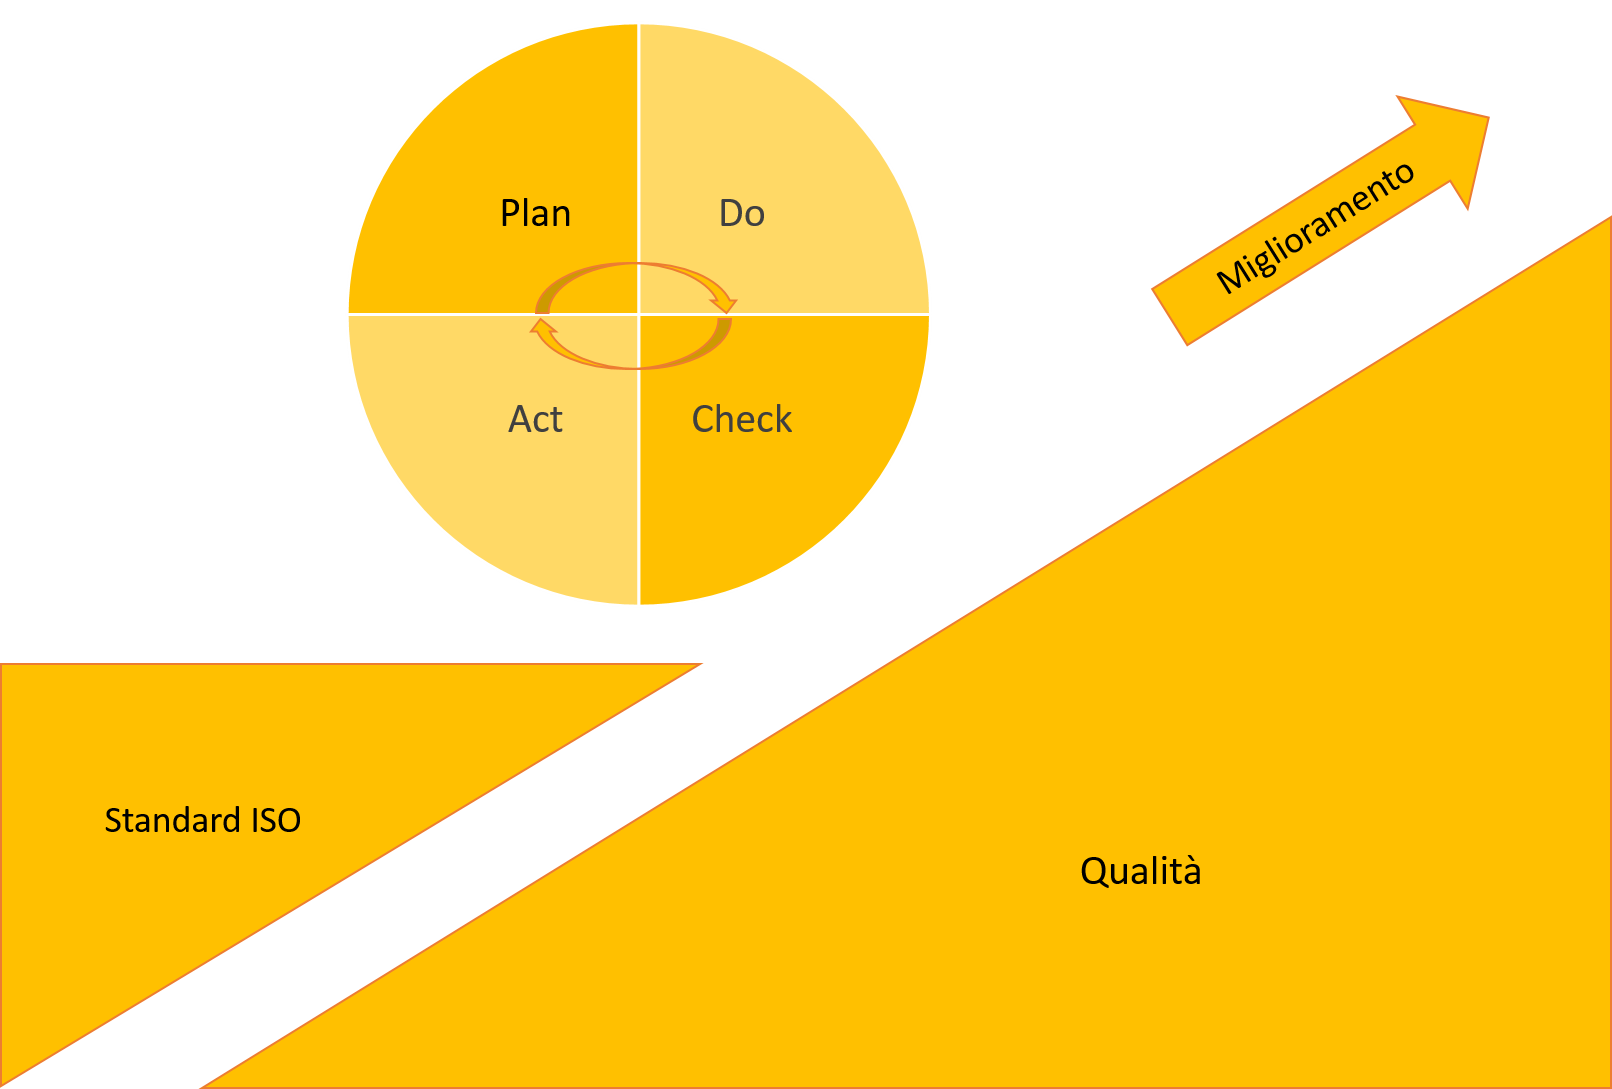
\includegraphics[width= 11.5cm]{immagini/pdca.png}
	\caption{Ciclo di Deming}
\end{figure}

Il ciclo PDCA\G\ è suddiviso in 4 fasi:

\begin{itemize}
	\item \textbf{Plan:} fase di pianificazione che definisce:
\begin{itemize}
	\item[-] Gli obiettivi da raggiungere;
	\item[-] Come svolgere le attività per conseguirli, tenendo in considerazione le risorse disponibili e le scadenze;
	\item[-] Le responsabilità di chi va ad eseguire le attività;
	\item[-] Le metriche per valutare i processi.
\end{itemize}
	
	\item \textbf{Do:} fase di implementazione ed esecuzione delle strategie progettate nella fase precedente;
	
	\item \textbf{Check:} fase di verifica nella quale vengono controllati i risultati della fase precedente (secondo le metriche fissate nella fase \textit{Plan}) e in cui si confrontano i prodotti effettivi con quelli attesi;
	
	\item \textbf{Act:} fase che prevede il miglioramento dei processi: utilizzando i risultati della verifica, si progettano modifiche ai processi per migliorarli. Nello svolgimento di questa attività viene tenuto conto delle \textit{best practice\G}. Tutte le decisioni prese in questa fase vengono implementate a partire dalla successiva fase di \textit{planning}.
\end{itemize}
Lo scopo di questo ciclo è il continuo incremento qualitativo del processo di sviluppo e, conseguentemente, del prodotto. L'appoggio agli \textit{standard} e alle \textit{best practice} permette di consolidare il livello raggiunto e di non retrocedere. Il miglioramento può progredire infinitamente nel tempo, data l'assenza di limiti fissati.

\subsection{Standard ISO/IEC 9126}

Lo standard ISO\G/IEC\G\ 9126 è stato creato con lo scopo di descrivere gli 
obiettivi qualitativi del prodotto e definire le metriche che possono misurare 
il raggiungimento di tali obiettivi. Vi sono infatti dei criteri suddivisi in tre 
aree:

\begin{itemize}
	\item \textbf{Qualità in uso:} è la qualità del prodotto \textit{software} 
	visto dall'utilizzatore, che ne fa uso in uno specifico contesto;
	\item \textbf{Qualità esterna:} è la qualità del prodotto 
	\textit{software} visto dall'esterno, quando viene eseguito e testato in un 
	ambiente di prova;
	\item \textbf{Qualità interna:} è la qualità del prodotto 
	\textit{software} visto dall'interno, facendo riferimento a 
	caratteristiche implementative, come l'architettura o il codice che ne 
	deriva.
\end{itemize}
Essendo inizialmente impossibile testare la qualità in uso, si è deciso di 
focalizzarsi sulla qualità interna ed esterna. Nello standard sono previste sei 
caratteristiche qualitative principali, suddivise a loro volta in 
sottocategorie che possono essere misurate quantitativamente:

\begin{itemize}
	\item \textbf{Funzionalità:} capacità del prodotto di fornire le funzioni richieste
	\begin{itemize}
		\item \textbf{Idoneità:} capacità del prodotto di fornire un insieme di funzioni appropriate per un'attività;
		\item \textbf{Accuratezza:} capacità del prodotto di fornire risultati 
		coerenti e corretti a seconda del grado di precisione richiesto;
		\item \textbf{Interoperabilità:} capacità interattiva del prodotto 
		\textit{software} con uno o più sistemi;
		\item \textbf{Sicurezza:} capacità del prodotto \textit{software} di 
		proteggere i dati e le informazioni, e a consentire solo a sistemi 
		autorizzati di fare modifiche;
		\item \textbf{Conformità funzionale:} capacità del prodotto 
		\textit{software} di essere aderente allo standard in materia di 
		funzionalità.
	\end{itemize} 
	
	\item \textbf{Affidabilità:} capacità del prodotto di garantire un livello di prestazioni adeguato
	\begin{itemize}
		\item \textbf{Maturità:} capacità del \textit{software} di evitare 
		fallimenti causati da errori;
		\item \textbf{Tolleranza agli errori:} capacità del \textit{software} 
		di mantenere un adeguato livello di prestazioni nonostante errori o 
		violazioni dell'interfaccia;
		\item \textbf{Capacità di recupero:} capacità del \textit{software} di 
		ristabilire un livello di \textit{performance} adeguato e di recuperare 
		dati in caso di errori;
		\item \textbf{Conformità di affidabilità:} capacità del prodotto 
		\textit{software} di essere aderente allo standard in materia di 
		affidabilità.
	\end{itemize}
	
	\item \textbf{Usabilità:} capacità del prodotto di essere facilmente comprensibile ed usabile, e di risultare interessante per l'utente
	
	\begin{itemize}
		\item \textbf{Intelligibilità:} capacità del \textit{software} di 
		permettere all'utente di capire se il prodotto è adeguato e se possa 
		essere utilizzato per dei compiti particolari;
		\item \textbf{Apprendibilità:} capacità del \textit{software} di 
		consentire all'utente di imparare ad utilizzare le sue funzionalità;
		\item \textbf{Operabilità:} capacità del \textit{software} di 
		consentire ai suoi utenti di essere usato;
		\item \textbf{Attrattività:} capacità del \textit{software} di creare 
		interesse negli utenti;
		\item \textbf{Conformità di usabilità:} capacità del 
		\textit{software} di essere aderente allo standard in materia di 
		usabilità.
	\end{itemize}
	
	\item \textbf{Efficienza:} capacità del prodotto di fornire prestazioni adeguate a seconda delle risorse utilizzate
	\begin{itemize}
		\item \textbf{Comportamento temporale:} capacità del \textit{software} 
		di dare una risposta in tempi di elaborazione adeguati, quando svolge 
		le sue funzionalità;
		\item \textbf{Utilizzo di risorse:} capacità del \textit{software} di 
		utilizzare le risorse adeguate per la sua esecuzione;
		\item \textbf{Conformità di efficienza:} capacità del 
		\textit{software} di essere aderente allo standard in materia di 
		efficienza.
	\end{itemize}
	
	\item \textbf{Manutenibilità:} capacità del prodotto di essere modificato e 
	aggiornato. Tali modifiche o aggiornamenti possono rispecchiare correzioni, 
	miglioramenti o adattamenti del \textit{software} nei confronti di cambiamenti ambientali, 
	di specifiche o delle funzionalità
	\begin{itemize}
		\item \textbf{Analizzabilità:} capacità del \textit{software} di poter 
		essere studiato per cercare difetti;
		\item \textbf{Modificabilità:} capacità del \textit{software} di 
		consentire l'implementazione di una qualche modifica;
		\item \textbf{Stabilità:} capacità del \textit{software} di evitare 
		errori o fallimenti causati da una o più modifiche;
		\item \textbf{Testabilità:} capacità del \textit{software} di 
		permettere la validazione di una versione modificata del 
		\textit{software};
		\item \textbf{Conformità di manutenibilità:} capacità del prodotto 
		\textit{software} di essere aderente allo standard in materia di 
		manutenibilità.
	\end{itemize}
	
	\item \textbf{Portabilità:} capacità del \textit{software} di poter essere 
	spostato in vari ambienti di lavoro
	\begin{itemize}
		\item \textbf{Adattabilità:} capacità del \textit{software} di essere 
		adattato a diversi ambienti senza necessitare di modifiche;
		\item \textbf{Installabilità:} capacità del \textit{software} di poter 
		essere installato in ambienti differenti;
		\item \textbf{Coesistenza:} capacità del \textit{software} di 
		coesistere con altri \textit{software} indipendenti condividendo delle 
		risorse;
		\item \textbf{Sostituibilità:} capacità del \textit{software} di poter 
		sostituire un \textit{software} simile che abbia le stesse funzionalità 
		e che sia nello stesso ambiente;
		\item \textbf{Conformità di portabilità:} capacità del prodotto 
		\textit{software} di essere aderente allo standard in materia di 
		portabilità.
	\end{itemize}
	
\end{itemize}
\newpage